\documentclass[11pt,a4paper]{book}
\usepackage[utf8]{inputenc}
\usepackage{float}
\usepackage{tikz}
\usepackage{graphicx}
\graphicspath{ {./images/} }
\usepackage{fancyhdr}
\usepackage[spanish]{babel}
%\usepackage{csquotes}
\usepackage[left=2cm,right=2cm,top=2cm,bottom=2cm]{geometry}\usepackage[backend=bibtex]{biblatex}
\addbibresource{bibliografia.bib}



\title{
{Borrador TFG Vihrtual-App}\\
{\large Universitat Politècnica de València}\\
%{\includegraphics{university.jpg}}
}
\author{Joan Ciprià Moreno Teodoro}
\date{Gandía, 2021}

\fancyhf{}
\cfoot{\thepage}
\pagestyle{fancy}

\begin{document}

\maketitle

\chapter*{Resumen}
[TODO: Resumen de máximo 200 palabras]
\\
\\
\textbf{Palabras clave:} chatbots, virus de la inmunodeficiencia humana, lenguaje natural, inteligencia artificial, salud.

\chapter*{Abstract}
[TODO: Resumen de máximo 200 palabras en inglés]
\\
\\
\textbf{Keywords:} chatbots, human immunodeficiency virus, natural language, artificial inteligence, health. 

\tableofcontents

\chapter{Introducción}
\input{chapters/introducción}

\chapter{Marco Teórico}
\input{chapters/marco_teórico}

\chapter{Desarrollo de la Propuesta}

\section{Análisis de requisitos}
 


\section{Solución propuesta}
Después de analizar detenidamente los requisitos se procede a detallar la solución propuesta para el desarrollo de Vihrtual-App.

\subsection{Tratamientos del dataset}

\subsection{Aspectos técnicos}
Eklegmos rasa, cumple con el capitulo anterior

\subsection{Personalidad}
caracteristicas sociales del bot, uso de emojis, efectos visuales, avatar

\subsection{Distribución}
Teniendo en cuenta el carácter del servicio se propone que el chatbot se ponga a disposición del público a través de una web de libre acceso y sin requerir registro. El objetivo es facilitar a los usuarios el acceso  y esta opción hará que cualquier persona pueda acceder al servicio sin necesidad de introducir ningún dato personal ni instalar ninguna aplicación en su terminal. \\

Para aquellos usuarios que lo deseen se empaquetará la web en una aplicación tanto para \textit{Android} como para \textit{iOS} utilizando el framework \textit{Capacitor}. Esto permitirá que aquellos usuarios interesados puedan instalar el servicio desde las tiendas de aplicaciones habituales en sus dispositivos móviles.\\

\subsection{Roadmap}
Siguiendo la metodología \textit{Scrum} se propuso una ruta de desarrollo (ver figura \ref{fig:roadmap desarrollo}) centrada en la obtención de un producto mínimo via	ble lo antes posible. Para ello primeramente se realizarían los diseños del chatbot, se organizaría la información recibida y se trabajaría para la obtención de un \textit{PMI} en versión web. A partir de ese punto se publicaría una versión de prueba del \textit{bot} para con la obtención de datos reales realizar distintas iteraciones sobre el producto hasta conseguir el resultado deseado. Una vez se alcanzara el nivel de madurez requerido, la web se empaquetaría como \textit{app} para móvil y se publicaría.\\

\begin{figure}[htbp]
\centering
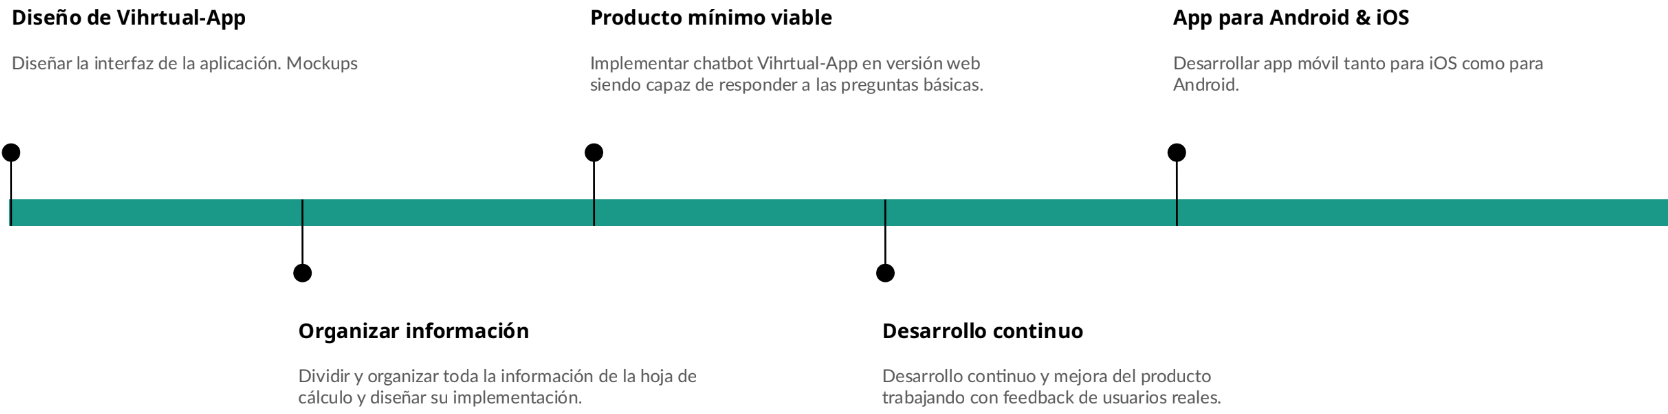
\includegraphics[scale=0.4]{../images/roadmap.png} 
\caption{\textit{Roadmap} propuesto para el desarrollo de Vihrtual-App}
\label{fig:roadmap desarrollo}
\end{figure}

Este propuesta fue presentada en una reunión con los colaboradores la Unidad de Enfermedades Infecciosas del Hospital General de Elche para obtener su aprobación. Las diapositivas se pueden encontrar en los documentos anexos a este trabajo.\\

\section{Diseño}
\input{chapters/desarrollo_propuesta/diseño}

\section{Implementación}
\input{chapters/desarrollo_propuesta/implementación}

\chapter{Pruebas de validación}
En esta sección se muestran las distintas pruebas de validación\\
 

\section{Evaluación del modelo NLU}
split nlu 

\section{Evaluación de usabilidad}
Finalmente, se ha realizado una prueba de usabilidad a la aplicación para detectar posibles problemas y corregirlos. Los participantes fueron captados a través de una invitación por email enviada por los tutores del TFG. El correo incluía un breve texto indicando a los participantes que probaran durante unos minutos el chatbot y que posteriormente realizaran un cuestionario a través de un link. Todos los participantes que realizaron el cuestionario han sido incluidos en los resultados. En total, 10 adultos de entre 16 y 60 años participaron en la prueba durante un periodo de 7 días.\\

Para este estudio se han utilizado los cuestionarios validados \textit{System Usability Scale} (SUS) \cite{dirtySUS} y \textit{Chatbot Usability Questionnaire} (CUQ) \cite{cuq}. SUS es un cuestionario genérico diseñado para obtener una evaluación general y rápida sobre la usabildiad de una determinada aplicación \cite{dirtySUS}. Se compone de 10 sentencias sobre las cuales los usuarios deben valorar en una escala del 1 al 5 su total disconformidad (1) o total conformidad (5). Se utilizó una versión del SUS traducida al español y validada \cite{spanishSUS}.\\

Por otro lado, CUQ es un cuestionario de usabilidad específico que evalúa la personalidad, la inteligencia, el entendimiento, la navegación y el manejo de errores de un chatbot \cite{cuq}. CUQ está diseñado para ser comparable al SUS (utiliza la misma escala de valoración) pero utilizando 16 sentencias específicas para chatbots. Para su uso, se realizó una traducción lo más fiel posible al español.\\

\subsection{Cálculo de puntuaciones}
Se utilizó la hoja de cálculo de la puntuación de SUS \cite{susSpread} para calcular las puntuaciones del SUS sobre 100. La fórmula para este cálculo se muestra en la ecuación 1.\\


donde n=número de sujetos (cuestionarios), m=10 (número de preguntas), qi,j=puntuación individual por pregunta por participante, norma=2,5.\\



Las puntuaciones del CUQ se calcularon sobre 160 utilizando la fórmula de la ecuación 2, y luego se normalizaron para dar una puntuación sobre 100, permitiendo así la comparación con SUS. \\


donde m = 16 (número de preguntas) y n = puntuación de la pregunta individual por participante \cite{cuq}.\\

\subsection{Resultados}


\chapter{Conclusiones}
\input{chapters/conclusión}

\printbibliography[heading=bibnumbered]

\appendix
\chapter{Apéndice}
\input{chapters/apéndice}

\end{document}